\labsection{ПРИЛОЖЕНИЕ}

\labsection{Газовый разряд}

Под термином <<газовый разряд>> обычно понимают все явления и процессы,
связанные с протеканием электрического тока через газ.

Само название <<разряд>> произошло от названия медленно протекающего
процесса потери заряда заряженными металлическими телами,
расположенными на подставке из изолятора, что наблюдалось ещё в
XVI~веке. Позднее Кулон экспериментально доказал, что заряд стекает
с проводника через воздух, а не через подставку из изолятора.
Разряд при низких давлениях воздуха (порядка 1~мбар) открыл и исследовал
Фарадей~--- этот разряд стал известен как \term{тлеющий}. В конце XIX~века
исследование проводимости разреженных газов привело Дж.Дж.~Томсона к
открытию первой элементарной частицы~--- электрона, а дальнейшие исследования
физики газового разряда во многом послужили экспериментальной основой
атомной и квантовой физики.

% Основателем физики собственно газового разряда считается Таунсенд, ученик
% Дж.~Дж.~Томсона, создавший в начале XX~века
% теорию пробоя газа и установивший закономерности ионизации. Следующий
% принципиальный вклад в физику газового разряда был
% внесён Ленгмюром, который вместе с Тонксом в 1928~году, исследуя газовый разряд
% низкого давления, ввёл такое
% фундаментальное понятие физики, как плазма,
% а также развил методы исследования плазмы, в частности, метод зондов.

Современная физика термин \term{газовый разряд} трактует в более широком
смысле. Это~--- не только процесс протекания тока через газ, но и любой процесс
возникновения ионизации газа под действием приложенного электрического поля.
При этом поле может быть не только постоянным во времени,
но и быстропеременным~--- высокочастотным (ВЧ-разряд, мегагерцы),
сверхвысокочастотным (СВЧ-разряд, гигагерцы) и даже оптического диапазона
(оптический разряд). Отдельно можно отметить пучково-плазменный разряд (ППР),
загорающийся при прохождении электронного пучка через газ малой плотности
вследствие возникновения в такой системе плазменных колебаний СВЧ-диапазона.
% Термины \important{горение} и \important{зажигание} получили распространение
% применительно к газовому разряду, потому что при достаточно сильной ионизации
% газ светится.

Разряды в постоянном поле разделяют на \term{несамостоятельные} и
\term{самостоятельные}. Дело в том, что при нормальных
условиях газы состоят в основном только из электрически нейтральных атомов и
молекул и практически не проводят ток.
% , по сути, являются диэлектриками, то есть
% изоляторами, поэтому через них не может проходить сколько-нибудь
% заметный электрический ток.
Проводниками могут быть только хоть в какой-то мере ионизованные газы.
Носителями тока в могут быть положительные и отрицательные ионы и электроны.
Ионы в газах могут возникать в результате действия различных
источников энергии, например: ультрафиолетового излучения или рентгеновских лучей,
космического излучения, лучей радиоактивных загрязнений,
столкновений атомов газа с электронами и другими частицами, энергия
которых превышает потенциал ионизации атомов газа.

Предположим, что ионы в газовом проводнике создаются исключительно внешним
источником. Тогда при прекращении действия этого <<ионизатора>> ток и,
следовательно, разряд прекращаются. Такой разряд называется
\term{несамостоятельным}.

\begin{figure}[h]
    \centering
%     \psfragfig[width=0.6\textwidth]{Images/Chapter_5/v5_2}{%
%   \psfrag{u}{$U$}
%   \psfrag{i}{$I$}
%   \psfrag{0}[rt]{0}
%   \psfrag{a}[br]{А}
%   \psfrag{b}{Б}
%   \psfrag{v}{В}
%   \psfrag{g}{Г}
%     \psfrag{d}{Д}}
    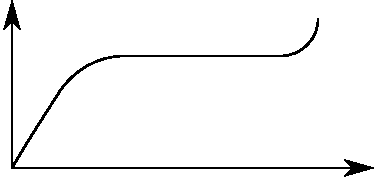
\includegraphics[width=0.4\textwidth]{Chapter_5/v5_2.pdf}
    \caption{Вольт-амперная характеристика несамостоятельного газового разряда}
    \figmark{Non-self discharge VAC}
\end{figure}

Типичная кривая, отображающая связь между током через газовый промежуток и
напряжением на нём для несамостоятельного разряда показана на
рис.~\figref{Non-self discharge VAC}. С повышением напряжения
на газовом промежутке ток сначала возрастает (кривая ОА), а потом достигает
насыщения и остаётся практически постоянным (участок АБ), что соответствует
полному вытягиванию на электроды зарядов, создаваемых внешним ионизатором.

\begin{wrapfigure}{o}{0.36\textwidth}
\centering
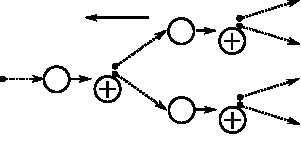
\includegraphics[width=\linewidth]{Chapter_5/v5-avalanche.pdf}
\caption{Схема образования электронной лавины}
\figmark{avalanche}
\end{wrapfigure}

При дальнейшем повышении напряжения ток снова начинает возрастать (участок БВ).
Это значит, что имеющиеся ионы, и прежде всего электроны, за период между двумя
последовательными столкновениями набирают такую энергию, что возникнет
\important{столкновительная ионизация}, то есть рождение новых,
\important{вторичных ионов}. При этом,
если количество выбитых при столкновениях электронов достаточно велико,
возникают и развиваются \term{электронные лавины},
то есть происходит <<размножение>> носителей и усиление тока,
часто называемое \term{газовым усилением} (см. рис.~\figref{avalanche}).
% При каком значении поля наступит размножение, зависит от давления
% газа и энергии, необходимой для ионизации
% данной молекулы (потенциала ионизации).
% В результате усиления концентрация ионов возрастает до величины, которая линейно
% или даже более сильно зависит от первичной ионизации.
При этом разряд остаётся несамостоятельным: если убрать первичный источник
ионизации, пропадут и лавины.

В достаточно сильном электрическом поле проводимость газа может возрасти
скачком~--- возникает \term{пробой}.
% Соответствующее напряжение на газовом промежутке называется
% \term{напряжением пробоя} ( или \important{напряжением зажигания}).
Если после возникновения пробоя убрать внешний ионизатор, то разряд не
прекращается. Разряд переходит в режим \term{самостоятельного разряда}:
ионизация поддерживается процессами в самом разряде.

\paragraph{Критерий Таунсенда зажигания разряда.}
Рассмотрим модель перехода несамостоятельного разряда в самостоятельный,
предложенную Таунсендом.
Определим \term{коэффициент объёмной ионизации} $\alpha$ ---
количество вторичных электронно-ионных пар, образуемых одним электроном
на единице длины пути.
Этот коэффициент зависит от плотности газа
(плотность определяет число соударений)
% растёт с увеличением давления $P$ газа
и растёт с увеличением напряжённости электрического поля $E$
(так как при этом увеличивается энергия электронов).
% , $\alpha=\alpha(P,\,E)$.

\begin{figure}[h!]
    \centering
%     \psfragfig[width=0.5\textwidth]{Images/Chapter_5/v5_3}{%
%   \psfrag{0}{0}
%   \psfrag{a}[rb]{$x$}
%   \psfrag{D}[cb]{$dx$}
%   \psfrag{d}[rb]{$d$}
%     \psfrag{x}{$X$}}
    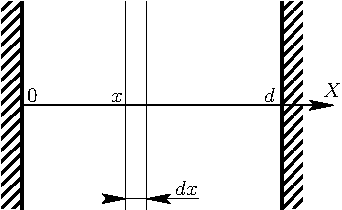
\includegraphics[width=0.4\textwidth]{Chapter_5/v5_3.pdf}
    \caption{К выводу критерия Таунсенда зажигания разряда}
    \figmark{Townsend criterion}
\end{figure}

Рассмотрим, как происходит ионизация в газовом промежутке между плоскими
электродами~--- катодом и анодом (рис.~\figref{Townsend criterion}). На
расстоянии~$x$ от катода в слое толщины $dx$ один электрон создаёт $\alpha dx$
пар ионов. Если со стороны катода в этот
слой втекает электронный ток~$I_e$, то в слое он возрастёт на величину
\begin{equation*}
\eqmark{dI}
dI_e=I_e\alpha dx.
\end{equation*}
Предположим, что токи в системе достаточно малы, так что в газовом промежутке
не накапливаются существенные объёмные заряды --- тогда электрическое поле~$E$,
а следовательно и коэффициент~$\alpha$, не зависят $x$.
% (это справедливво при малых токах, когда в газе нет объёмных зарядов, и,
% следовательно, $E$ не зависит от $x$).
Тогда интегрируя \eqref{dI} при $\alpha=\const$, находим:
\begin{equation*}
	I_e(x)=I_e(0)e^{\alpha x},
\end{equation*}
где $I_e(0)$~--- электронный ток, втекающий в систему с катода.

Видно, что на аноде ($x=d$) ток возрастает в $e^{\alpha d}$~раз.
% Например, при
% $\alpha=3~\text{см}^{-1}$ и $d=3$~см ток возрастёт приблизительно
% на 4 порядка.
Это и есть режим \important{газового усиления}, то есть размножения
электронно-ионных пар вследствие развития
электронных лавин. Однако при этом разряд ещё не обязательно переходит в режим
самостоятельного. Чтобы разряд не прекращался, нужно,
чтобы ток с катода $I_e(0)$ поддерживался \important{самим разрядом},
то есть чтобы образовалась \important{положительная обратная связь}.
Такая связь может установиться только благодаря потоку частиц, двигающихся
из разряда в обратном направлении --- к катоду. В модели Таунсенда это~---
положительные ионы и излучение. Далее для простоты будем учитывать только положительные ионы.

Полный ток через любое поперечное сечение разряда одинаков.
Он складывается из электронной и ионной составляющих.
Полный ток на аноде равен чисто электронному току $I_e(d)$,
а ионный ток на катоде $I_i(0)$ равен
\begin{equation*}
	I_i(0)=I_e(d)-I_e(0)=I_e(0)(e^{\alpha d}-1).
\end{equation*}
Пусть теперь каждый попавший на катод ион выбивает из него в среднем
$\gamma$ вторичных электронов
($\gamma$~--- \term{коэффициент вторичной ионно-электронной эмиссии}).
Тогда из катода пойдёт ток этих вторичных электронов $I_2$:
\begin{equation*}
	I_2=\gamma I_i(0)=\gamma I_e(0)(e^{\alpha d}-1).
\end{equation*}
Полный электронный ток из катода складывается из тока $I_1$,
образуемого внешним ионизатором, и тока вторичных электронов $I_2$:
\begin{equation*}
	I_e(0)=I_1+I_2=I_1+\gamma I_e(0)(e^{\alpha d}-1),
\end{equation*}
так что
\begin{equation*}
	I_e(0)=\frac{I_1}{1-\gamma(e^{\alpha d}-1)}.
\end{equation*}
Таким образом, полный ток через газовый промежуток $I$ будет равен
% равный электронному току через анод, будет равен
\begin{equation}
    \eqmark{taunsendI}
	I=I_e(d)=I_e(0)e^{\alpha d}=\frac{I_1e^{\alpha d}}{1-\gamma(e^{\alpha
d}-1)}.
\end{equation}

С повышением напряжения на газовом промежутке, то есть с ростом электрического
поля $E$, растут коэффициенты $\alpha$ и $\gamma$, и ток возрастает.
Разряд тем не менее остаётся несамостоятельным: при $I_1=0$ ток разряда
обращается в нуль. Однако при достижении некоторого значения поля
знаменатель \eqref{taunsendI} обратится в нуль,
а ток~--- в бесконечность при любом сколь угодно малом значении $I_1$.
% , так что внешний ионизатор можно вообще убрать.
Это и есть \important{переход от несамостоятельного разряда к
самостоятельному}, или \term{наступление пробоя}, а его
условие~--- \term{критерий Таунсенда} --- имеет вид
\begin{equation}
    \eqmark{taunsend}
	\gamma(e^{\alpha d}-1)\ge 1.
\end{equation}
Если известны зависимости $\gamma(E)$ и $\alpha(E)$, из условия \eqref{taunsend}
можно определить \term{потенциал зажигания} разряда $U_{з}$
(\term{напряжение пробоя}).

Коэффициент $\gamma (e^{\alpha d}-1)$ можно назвать
\important{коэффициентом воспроизводства электронов} --- от одного электрона,
вылетевшего с катода, рождается $e^{\alpha d}-1$ ионов,
каждый из которых впоследствии выбивает с катода ещё $\gamma$ электронов.

На практике потенциал зажигания определяют из экспериментально измеренных
\term{кривых Пашена}: зависимости $U_{з}$ от произведения
давления $P$ на длину разрядного промежутка $d$: $U_{з}(Pd)$.
Типичная кривая Пашена приведена на рис.~\figref{Paschen curve}.
Кривая имеет минимум, поэтому для заданного $P$ имеется такая длина
$d_{\rm min}$ разрядного промежутка,
при которой потенциал зажигания и соответствующее ему поле минимальны
(это важно для структуры тлеющего разряда, см. ниже).

\begin{figure}[h!]
	\centering
%     \psfragfig[width=0.7\textwidth]{Images/Chapter_5/v5_4}{%
% 	\psfrag{P}[rb]{$P\cdot d$, см$\cdot$торр}
% 	\psfrag{V}[lb]{$U_{з}$, В}
% 	\psfrag{2}[tc]{\footnotesize2}
% 	\psfrag{4}[tc]{\footnotesize4}
% 	\psfrag{6}[tc]{\footnotesize6}
% 	\psfrag{a}[tc]{\small$10^{-1}$}
% 	\psfrag{b}[tc]{\small$10^0$}
% 	\psfrag{c}[tc]{\small$10^1$}
% 	\psfrag{d}[tc]{\small$10^2$}
% 	\psfrag{e}[tc]{\small$10^3$}
% 	\psfrag{A}[rc]{\small$10^2$}
% 	\psfrag{B}[rc]{\small$10^3$}
% 	\psfrag{C}[rc]{\small$10^4$}
% 	\psfrag{3}[rc]{\footnotesize2}
% 	\psfrag{5}[rc]{\footnotesize4}
%     \psfrag{7}[rc]{\footnotesize6}
% }
	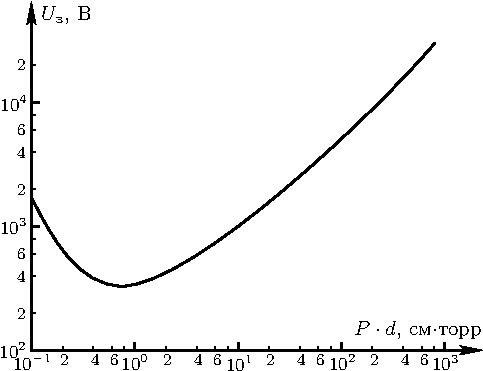
\includegraphics[width=0.7\textwidth]{Chapter_5/v5_4.pdf}
	\caption{Зависимость потенциала зажигания $U_\text{з}$ от произведения
давления~$P$ на~длину $d$ разрядного промежутка (кривая Пашена) для воздуха}
	\figmark{Paschen curve}
\end{figure}

%  Напомним, что в модели
% Таунсенда поле в промежутке однородно и не искажается объёмными зарядами, что
% верно только для разряда с очень маленьким
% током. Такой самостоятельный разряд известен как \term{тёмный
% таунсендовский разряд}.

Описанный процесс пробоя называют \term{таунсендовским}. Существуют и другие
механизмы: например, в газах высокого давления (больше атмосферного) и при
больш\'{и}х длинах промежутков реализуется \term{стриммерный}
(или \term{искровой}) механизм, а возникающий в результате такого пробоя
нестационарный разряд известен как \term{искровой}. Примером такого разряда
является молния. Для искрового разряда характерны сильные поля и коротки времена.
Разряд происходит по треку предварительно образовавшегося
канала --- стримера. За его образование отвечают множественные электронные лавины,
однако в отличие от таунсендского разряда, начало лавине даёт ионизация
фотоном, испущенным предыдущей лавиной. Поскольку фотоны, в отличие
от электронов, распространяются со скоростью света, развитие стриммера идёт
намного быстрее, чем единичной электронной лавины.

\paragraph{Вольт-амперная характеристика газового разряда.}

В широком смысле термин \term{электрический пробой} означает превращение
изолятора в проводник в результате приложения к
нему достаточно сильного поля. Для газа это означает переход в ионизованное
состояние. При этом возрастание тока
приводит к ещё большему возрастанию концентрации ионов, что приводит к
возрастанию проводимости и, следовательно, к
понижению напряжения, необходимого для поддержания такого тока.

Будем характеризовать электрические свойства газового промежутка,
заключённого между двумя помещёнными в газ электродами,
\term{вольт-амперной характеристикой} (ВАХ). Так принято делать
всегда в случае нелинейной зависимости тока через
проводящий элемент от приложенного напряжения.

Введём понятие \term{дифференциального
сопротивления} как производную по току от напряжения:
\begin{equation}
    \eqmark{Rdiff}
R_{диф} = \frac{dU}{dI}.
\end{equation}
Для газового разряда имеет место новое (не свойственное обычным
проводникам) явление~---
\term{отрицательное дифференциальное сопротивление},
$R_{диф} < 0$
(напомним, что для проводников, подчиняющихся
закону Ома, например металлов, $R_{диф}$
равно обычному сопротивлению и всегда положительно).

\begin{wrapfigure}{o}{0.4\textwidth}
    \centering
%     \psfragfig[width=0.6\textwidth]{Images/Chapter_5/v5_5}{%
%   \psfrag{A}[cc]{$A$}
%   \psfrag{V}[cc]{$V$}
%   \psfrag{R}{$R$}
%     \psfrag{E}[cb]{$\mathcal{E}$}}
    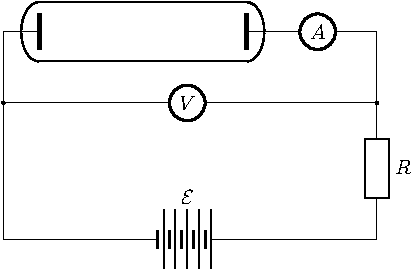
\includegraphics[width=0.4\textwidth]{Chapter_5/v5_5.pdf}
    \caption{Схема для снятия ВАХ газового промежутка}
    \figmark{Gas gap VAC scheme}
\end{wrapfigure}

Экспериментально ВАХ газового проводника~--- например, промежутка между двумя
электродами, помещёнными в стеклянную трубку, заполненную газом,~---
можно снять с помощью схемы, представленной на рис.~\figref{Gas gap VAC scheme}.
Цепь содержит источник постоянного напряжения $\mathcal{E}$,
% ,величину которого можно изменять в пределах примерно от 100~В до нескольких кВ,
и переменное сопротивление $R_0$, называемое <<балластным>>, или <<нагрузочным>>.
Это сопротивление необходимо для ограничения тока в цепи и стабилизации разряда
на участках с отрицательным дифференциальным сопротивлением. Дело в том, что
при $R_{диф} < 0$ разряд \important{неустойчив} и ток имеет тенденцию неограниченно
нарастать.

Меняя $\mathcal{E}$ и $R_0$ с помощью схемы на рис.~\figref{Gas gap VAC scheme}
можно получить любой возможный режим протекания тока через исследуемый газовый проводник.
На плоскости $I$--$U$ такой режим определяется точкой пересечения ВАХ $U(I)$
с <<нагрузочной>> прямой $U=\mathcal{E}-IR_0$.
Для устойчивости разряда суммарное дифференциальное сопротивление такой цепи должна быть
положительным: $\frac{dU}{dI} + R_0 > 0$. Иными словами, в точке пересечения с ВАХ
нагрузочная прямая должна иметь больший наклон,
чем участок кривой ВАХ разряда (рис.~\figref{Neon discharge VAC}),
что всегда можно обеспечить выбором достаточно большого $R_0$.

\begin{figure}[h!]
    \centering
    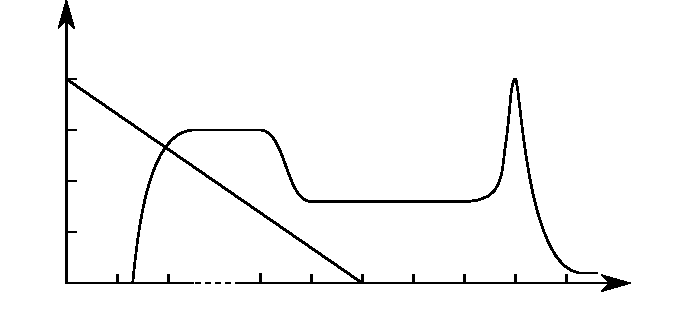
\includegraphics[width=0.8\textwidth]{Chapter_5/v5_6.pdf}
    \caption{ВАХ разряда в неоне при давлении 1 тор. Нагрузочная прямая проходит через область тлеющего разряда. Шкала по оси абсцисс --- логарифмическая}
    \figmark{Neon discharge VAC}
\end{figure}

Вид ВАХ для конкретного газового проводника зависит от ряда условий, прежде
всего от давления газа. На рис.~\figref{Neon discharge VAC} представлен пример
полученной экспериментально ВАХ разряда в неоне (при давлении $P\sim 1$~торр
между плоскими медными электродами площади 10~см$^2$, расположенными на
расстоянии 50~см), а также типичная нагрузочная прямая. Поскольку
здесь нет специального внешнего ионизатора (внешняя ионизация создаётся только
естественным радиоактивным излучением и космическими лучами), начальный участок
характеристики несамостоятельного разряда (участок ОА) соответствует столь
малым токам, что на графике его не удаётся изобразить. Характеристика
начинается сразу с участка АБ, соответствующего току насыщения и режиму
газового усиления. В точке В происходит пробой и начинается самостоятельный
разряд, который на всём горизонтальном участке характеристики ВГ соответствует
\term{тёмному таунсендовскому разряду}.

Участок характеристики ГДЕЖ соответствует \term{тлеющему разряду},
причём его падающая часть ГД называется \term{поднормальным тлеющим разрядом},
горизонтальная часть ДЕ~--- \term{нормальным тлеющим разрядом} и
остальная часть ЕЖ~--- \term{аномальным тлеющим разрядом}.

Нормальный тлеющий разряд обладает примечательным свойством самоорганизации:
при увеличении полного тока в разряде, его плотность остаётся практически
неизменной, меняется лишь площадь <<катодного пятна>>, из которого вытекает ток.
Меняя $\mathcal{E}$ или $R_0$, можно видеть, как светящееся пятно
на поверхности катода расширяется или сокращается.
При этом напряжение в разряде практически не меняется
(горизонтальный участок ВАХ на рис.~\figref{Neon discharge VAC}).

При полном заполнении катода дальнейшее увеличение тока будет возможно только за
счёт повышения интенсивности ионизации газа, что возможно только при повышении
напряжения. Разряд при этом переходит в режим аномального тлеющего разряда
(участок ЕЖ на ВАХ).

Далее идёт падающий участок ЖЗ. Он соответствует переходу к
\term{дуговому разряду}. Заметим, что при больш\'{и}х давлениях газа
(атмосферном и больше) после пробоя сразу устанавливается дуговой разряд.
Для дугового разряда характерны большие токи и сравнительно небольшие падения
напряжения. Электроны, поддерживающие ток, поставляются термоэмиссией
с горячего катода.

\paragraph{Пространственная структура тлеющего разряда.}
Отличительной характеристикой таунсендовского разряда
является \important{однородность} поля по длине промежутка, что обусловлено малостью тока
и отсутствием объёмных зарядов. Однако при большом токе разряда поле
перераспределяется после пробоя и почти полностью сосредотачивается у катода.
Это обусловлено образованием у катода положительного объёмного заряда за счёт
ионного тока (электронный ток у катода мал по сравнению с ионным). Кроме того,
остальная часть газового промежутка переходит в состояние с высокой
электропроводностью~--- образуется так называемый
\term{положительный столб}, замыкающий электрическую цепь.

\important{Самоподдерживающийся разряд с холодным катодом}, испускающим электроны
в результате вторичной эмиссии, называют \term{тлеющим}.
Он отличается от таунсендовского не только значительно б\'{о}льшим током,
но и, главным образом, существенной неоднородностью поля в разряде.

Почти вся приложенная разность потенциалов сосредоточена у катода на участке,
занятом объёмным зарядом, который называют \term{катодным слоем}.
Катодный слой~--- самая важная часть тлеющего разряда,
без него разряд существовать не может.
Напряжение на этом участке называют
\term{катодным падением напряжения} $V_{к}$ ($V_{к} \approx V$).
При этом толщина катодного слоя $d_{к}$ соответствует минимуму на кривой
Пашена \figref{Paschen curve}, где $V_{к}$ есть напряжение зажигания
на длине $d_{к}$. Тем самым реализуются условия для самоподдержания разряда
(критерий Таунсенда) при гораздо меньших напряжениях, чем при однородном поле
на всей длине газового промежутка.
Этим эффектом объясняется упомянутое выше явление постоянства плотности
тока в нормальном тлеющем заряде: при заданном $P$ толщина катодного
слоя $d_{к}$ и напряжение на нём $V_{к}$ фиксированы, следовательно
остаются неизменны напряжённость поля $E\sim V_{к}/d_{к}$, а значит
и плотность тока $j\propto E$.

% напряжение, необходимое для удовлетворения критерю Таунсенда,
% определяется
% устанавливается не на
% что поскольку напряжение на катодном слое и его толщина задаются условием
% минимума на кривой Пашена, они почти не меняются при заданном давлении газа.
% Следовательно, должна оставаться постоянной и плотность тока.



\begin{figure}[h!]
	\centering
    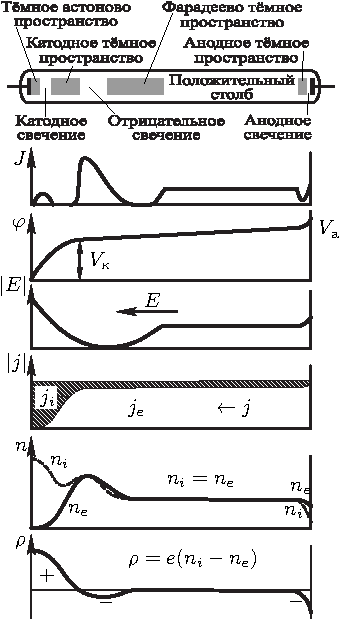
\includegraphics[width=0.5\textwidth]{Images/Chapter_5/v5_7.pdf}
	\caption{Структура тлеющего разряда и распределение по длине основных характеризующих его величин}
	\figmark{Glow discharge}
\end{figure}

На рис.~\figref{Glow discharge} представлена качественная картина тлеющего
разряда в длинной стеклянной трубке, а также приведены зависимости
основных величин, характеризующих разряд, от продольной координаты:
интенсивность свечения $J$, потенциал $\varphi$ и напряжённость $E$ электрического поля,
электронный $j_e$ и ионный $j_i$ токи,
электронная $n_e$ и ионная $n_i$ плотности и полная плотность объёмного заряда $\rho$.

Видно, что разряд состоит из ряда чередующихся светлых и тёмных поперечных
полос. Поскольку все процессы в разряде
связаны со столкновениями электронов с атомами газа, расстояния от катода до
этих полос определяются числом
укладывающихся на них длин пробега электронов. Поэтому характерные размеры полос
увеличиваются с уменьшением давления.
Непосредственно к катоду прилегает узкое \term{астоново пространство,}
затем идёт слой \term{кодного свечения}, а
затем~--- \term{тёмное катодное пространство}. Далее следует область
\term{отрицательного свечения,} переходящая в
\term{тёмное фарадеево пространство}. За ним начинается светящийся
\term{положительный столб}, заканчивающийся у анода
\term{тёмным анодным пространством}, переходящим на аноде в узкий слой
\term{анодного свечения}.

Как правило, самой яркой бывает область отрицательного свечения, имеющего для
воздуха голубоватый цвет, за что разряд и
получил своё название~--- тлеющий.

Качественно распределение свечения по длине разряда объясняется следующим
образом.

Электроны, выбиваемые из катода приходящими на него ионами, имеют энергию,
недостаточную для возбуждения атомов. Поэтому слой у катода~--- тёмный
(\term{астоново пространство}).

Далее электроны набирают достаточную
для этого энергию, и возникает первый светящийся слой,
\term{кодное свечение}.

Затем энергия электронов становится настолько
большой, что они в основном ионизуют, а не возбуждают атомы. Так образуется
\term{тёмное катодное пространство}, в котором происходит
основное размножение электронов и ионов.

Рождающиеся ионы движутся к катоду,
создавая большой положительный объёмный заряд. В конце тёмного
катодного пространства поля уже почти нет, оно экранировано объёмным зарядом,
зато образовалось очень много движущихся к аноду сравнительно медленных
электронов, которые снова возбуждают атомы. Так
начинается область \term{отрицательного свечения}.

Далее электроны растрачивают свою энергию (поле слабое) и возбуждение прекращается,
а свечение переходит в \term{тёмное фарадеево пространство}.

Основную часть разряда занимает квазинейтральный и практически однородный
по своим характеристикам \term{положительный столб} (см. ниже).
% В фарадеевом пространстве поле медленно нарастает до своего значения в
% , который можно рассматривать
% просто как участок омического проводника с электронной проводимостью.
% Здесь непрерывно происходят столкновения электронов с атомами,
% происходит их возбуждение, и положительный столб испускает свечение.

У анода ионов нет, электроны образуют отрицательный объёмный заряд,
создаётся небольшое \term{анодное падение потенциала}, в котором электроны
набирают энергию и вызывают \term{анодное свечение}.

Остановимся кратко на описании свойств положительного столба.
Этот участок газового разряда представляет собой пример
\important{низкотемпературной слабоионизированной неравновесной плазмы}.

Электрическое поле в нём однородно по длине,
как это имеет место в обычном омическом проводнике.
Под действием этого поля ток переносится в основном электронами.
% Состояние плазмы в положительном столбе практически не зависит от процессов в
% приэлектродных областях, и определяется только процессами внутри него.
Потери носителей тока (электронов) из-за диффузии к стенкам трубки и рекомбинации
компенсируются ионизацией. При этом необходимо электрическое поле $E$,
способное обеспечивать разгон электронов до соответствующей энергии.
Характерная энергия ионизации составляет несколько электрон-вольт,
поэтому температура электронов достигает значений $T_e \sim 10^4 - 10^5\;К$,
и существенно превосходит газовую температуру разряда $T$ (в газоразрядной трубке
$T$ будет практически совпадать с температурой стенок).
Столкновения горячих электронов с нейтральными атомами вызывают их возбуждение,
благодаря чему столб может испускать свечение.

В тлеющем разряде ВАХ положительного столба (и всего разряда) может быть
спадающей ($R_{диф}<0$, участок ГД и начало участка ДЕ на рис.~\figref{Neon discharge VAC}).
Это реализуется, когда потери электронов в основном обусловлены их диффузией к стенкам,
и объясняется нагревом газа: с увеличением тока плазма в центральной области
нагревается сильнее, её концентрация понижается, длина пробега электронов возрастает
--- и они получают возможность набирать необходимую для ионизации энергию при меньшем поле,
чем до нагрева. Следовательно, напряжение, необходимое для поддержания
такого тока, понижается. При достаточно больших токах увеличиваются
потери электронов за счёт рекомбинации, что требует увеличения поля ---
дифференциальное сопротивление вновь становится положительным
(конец участка ДЕ и участок ЕЖ рис.~\figref{Neon discharge VAC}).

% Случайные локальные перегревы, а также другие процессы, приводящие к появлению
% отрицательного дифференциального сопротивления, могут быть причиной развития
% различных \term{неустойчивостей}. Они могут вызывать вызвать стягивание
% разряда в токовый шнур (\term{контракция}). Этим объясняется переход
% аномального разряда в дуговой: катодное пятно уменьшается настолько,
% что катод в этом месте накаляется и начинается термоэмиссия.
% Другие неустойчивости
% ведут к образованию в положительном столбе поперечных слоёв, или
% \term{страт}, которые, как правило, движутся в
% продольном направлении.



\begin{lab:questions}

\item Назовите различные виды плазм в лаборатории, приложениях и природе.
% Параметры плазмы.

\item Что такое дебаевский радиус экранирования?

\item Дайте количественное определение понятия \term{плазма}.

\item Что такое плазменная частота? Выведите формулу для плазменной частоты.
Какие процессы в плазме характеризуются плазменной частотой?

\item Чем определяется потенциал зонда, погружённого в плазму?

\item Чем определяется зондовый ток насыщения для одиночного зонда? Для двойного
зонда?

\item Перечислите виды газового разряда.

\item Что такое вольт-амперная характеристика газового разряда?

\item Приведите основные параметры нормального тлеющего разряда. Является ли он
источником стацтонарной равновесной плазмы?

\item Опишите основной механизм зажигания тлеющего разряда.

\item Каков механизм зажигания разряда в высокочастотном поле?

\end{lab:questions}


\begin{lab:literature}

\item \textit{Сивухин Д.В.} Общий курс физики. Т.~III. Электричество.~--- М.:
Физматлит, 2003. --- Гл. IX.

\item \textit{Арцимович Л.А., Сагдеев Р.З.} Физика плазмы для физиков.~---
М.: Атомиздат, 1979.
% \item \textit{Кингсеп А.С.} Элементы физики плазмы: Учебно-методическое пособие.
% ~--- М:МФТИ 1985.

\item \textit{Райзер Ю.П.} Физика газового разряда.~--- Долгопрудный: Издательский
Дом Интеллект, 2009.

\item \textit{Чен Ф.} Введение в физику плазмы. Перевод с английского ~--- М.:
Мир, 1987.

\item \textit{Князев Б.А.} Низкотемпературная плазма и газовый разряд: Учебное
пособие/ Новосибирский государственный университет. ~--- Новосибирск, 2003.
\end{lab:literature}
